\chapter{INFORMATION SYSTEM IMPLEMENTATION}

\section{Development Methodology and Tools}

The rapid adaptation to the field's changing demands through high-quality code demonstrated the effectiveness of an agile methodology for developing this type of application. The software development process was broken down into four phases. Each phase was designed to produce specific results. The first phase included creating the complete infrastructure needed to build a static MongoDB database schema and developing base REST API controllers and secure authentication. Phase two consisted of producing the product menu and incoming orders (CRUD) features. The third and most difficult phase of the project was implementing real-time web socket synchronization that allows the kitchen interface to operate in a true real time mode. In addition, the fourth and final phase consisted mainly of refining the system and increasing its robustness against erroneous user interactions, such as accidental screen touches during high-pressure service. Additionally, full functional reporting was incorporated into the administrative reporting dashboards. The final phase provided the developers with an opportunity to test the system in a heavily loaded environment and to perform extensive load testing to ensure that the system will work correctly even when there are multiple users operating in the system. As part of our efforts to reduce potential problems with the system due to the continuous changes in functionality, we used a disciplined approach for managing our source code through a branching model. All source code changes were made in the main branch of our source control. The source code was always in a logically locked state. Proposed source code changes required approval via a merge request prior to being merged. Our feature-based development method was utilized to develop each phase of the project. This method allowed us to segregate unstable and incomplete code containing errors from the production version of the system while still providing a mechanism to demonstrate the capabilities of the system in a live environment.

\section{Backend Subsystem Development}

The backend is built using Express.js \cite{express} middleware to serve static content and handle base REST calls. However, the business logic behind orders (the main velocity) is in an event driven controller. Unlike MVC architectures, where there is separation of logic by layer and file name, this backend has an event handler that is designed to be as low-latency as possible. This design choice was made so that there would be no extra overhead from context switching between different layers of middleware while ingesting high-velocity orders.

\subsection{The Centralized Handler Pattern}

On the server side, there exists a holistic representation of the entire system as one large atomic workflow. There exists one single workflow that controls the life-cycle of an Order; no individual service can control the life cycle of an Order. 
Therefore, the overall architecture is designed to allow significant functions (stock-checks, deductions from the customers' accounts, and notifications sent to the customer) to be executed sequentially. Sequential execution of these important functions will eliminate the ability of two or more cashiers to attempt to purchase the last available item of stock at the exact same time (``a temporal race''). 
The back-office also maintains the same levels of data integrity guarantees under Peak Holiday Season Stress. Orders entered into the cashier interface are queued within a memory-based queuing system and then picked up from the queue atomically by the backend processing function. Regardless of whether the backend processing function is processing orders in First-In-First-Out (FIFO) order due to network jitter or some other reason, prior to executing any financial-related activity with regards to the disk, the backend processing function will perform recursive stock-level checks to verify that all of the required stock items are present in the system to complete the Order Item(s). The system throughput required by the System relies on highly efficient memory utilization, operating effectively within the constraints of standard commodity hardware (e.g., maintaining full operational capacity under peak load with less than 2GB of allocated RAM). Utilizing RAM for the system's critical validation business logic and the FIFO-style sequential processing eliminates row-locking of Database Tables and Deadlocks that can occur in SQL-based Systems when processing many transactions through a Shared Database. Listing 4.1 demonstrates a high-level conceptual model of the sequential logic employed during this atomic order processing phase (the complete technical implementation of this validation and execution sequence is provided in Appendix~\ref{sec:code_order_processing}).

\vspace{1em}
\noindent\textbf{Listing 4.1:} \textit{Order Processing logic demonstrating atomic stock validation and sequential execution.} \\
\vspace{-0.5em}
\begin{verbatim}
const processOrder = async (orderData) => {
  try {
    // 1. Validation: System state check
    const isActive = await verifySystemState();
    
    // 2. Atomic Stock Validation
    for (const item of orderData.items) {
      await validateIngredientAvailability(item);
    }

    // 3. Sequential Order Generation
    const orderNumber = await generateNextSequence();

    // 4. Persistence
    const order = new Order({ ...orderData, orderNumber });
    await order.save();

    // 5. Real-Time Broadcast
    broadcastToKitchen(order);
    
  } catch (error) {
    rejectOrderTransaction();
  }
};
\end{verbatim}
\vspace{1em}

\subsection{Real-time Communication Implementation}

Socket.io (the library) is used as the backbone of real-time capability. 
A global Socket.io instance is created in the backend server and is attached to the underlying HTTP server (the complete source code for the backend Socket.IO authorization setup is available in Appendix~\ref{sec:code_socket_auth}). 
All handshakes are intercepted before they can be converted into a real-time connection. 
When a handshake is intercepted, the secure token is extracted and decoded with a predefined key to identify a user. 
Room segmentation is utilized to reduce the amount of bandwidth used when multiple tablets are connecting in an event. 
Rather than sending all orders to each connected client device to the server, the server assigns each authenticated user a room based upon there role. 
For example, if a user with kitchen privileges connects to the kitchen room, then it will receive all the information for every order being prepared. If a cashier connects to the cashier room, then it will receive all the information about items that have been reached their minimum level of inventory.

\begin{figure}[htbp]
    \centering
    
\includegraphics[width=1.0\textwidth]{images/ch4_sequence_diagram.pdf}
    \caption{UML Sequence Diagram depicting the complete order lifecycle, from cashier submission through atomic server-side validation, database persistence, and real-time WebSocket broadcast to kitchen and waiter terminals.}
    \label{fig:sequence_diagram}
\end{figure}

\subsection{Security Middleware Integration}

The security logic of the system is multi-layered and built on top of one another through use of Express.js Middleware Functions. 
The base authentication middleware for Express accepts all incoming requests for the API, removes the Bearer Token from the HTTP Authorization header, then runs an algorithmic validation to verify the cryptographic signature of the Bearer Token. This layer is strictly responsible for \textit{authentication}---that is, confirming the identity of the requesting user.
After the authentication middleware function has validated the identity of the user, the gateway executes a second middleware function responsible for \textit{authorization}, which provides stricter Role-Based Access Controls. 
If the identified user does not have sufficient privileges to access the requested route, the gateway will deny access by rejecting the request with an error.

\section{Deep Technical Analysis of the Runtime Environments}

While high-level architectural design choices dictate the overall logical flow of the system, the raw execution speed, vertical scalability, and ultimate data safety of the proposed system are attributable directly to the underlying runtime engines chosen for this localized deployment.

\subsection{The V8 Engine Internals and Asynchronous I/O}

Node.js is faster than many other languages: The Google V8 JavaScript engine that Node.js uses to compile your code, on the fly, provides an environment that makes Node.js faster than most other programming languages. The V8 engine is designed to execute cloud-based applications at benchmark speeds. This is accomplished with just-in-time compilation (JIT) \cite{tilkov2010node}. With JIT, code is compiled at runtime to achieve the best performance with your code.

\begin{figure}[htbp]
    \centering
    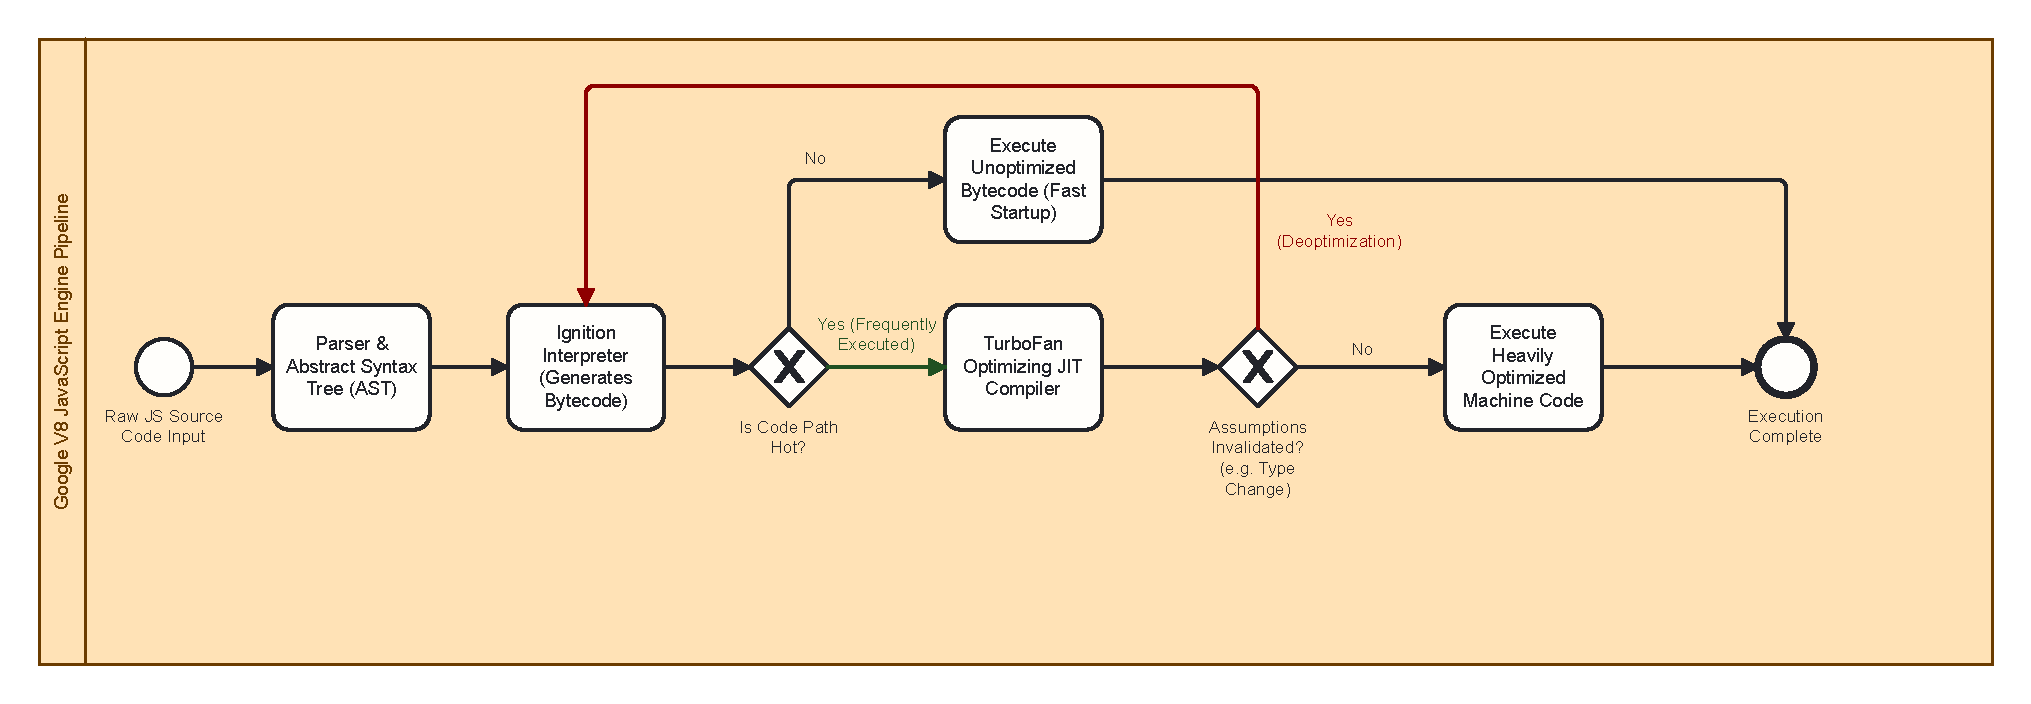
\includegraphics[width=0.8\textwidth]{images/ch4_v8_event_loop.pdf}
    \caption{The internal V8 Just-In-Time (JIT) compilation pipeline, actively identifying and deeply optimizing hot execution paths in real-time.}
    \label{fig:v8_compilation}
\end{figure}

Node.js also offers you more than just JIT compilation. In addition to internal deoptimization of your code and internal optimization of your code, once your code has a few ``hotspots'' (i.e., the order processing module of your application), where your application is operating at peak workload, the second optimizing compiler, TurboFan, will be launched in a separate thread and will run in the background. TurboFan will take the JavaScript code in the hotspots of your application and convert it into machine code optimized for your server's hardware architecture. 
V8 also performs a variety of optimizations including hidden classes and inline caching, to reduce the amount of memory used by your application. For example, since all of your Order and Product Entity Objects in your application have the same properties and structure, V8 can optimize how it allocates memory to your objects. In the logic of your application, instead of searching for the cost of the information in a hash table (which can be a relatively expensive operation), V8 can find the information it needs quickly at a predetermined memory address.

\subsection{Data Persistence with WiredTiger}

The system will use MongoDB with the WiredTiger storage engine, which has a high level of advanced capabilities that allow the system to provide transactional consistency similar to that of relational databases used in large enterprises.
WiredTiger is a high-performance storage engine that uses complex B-Tree algorithms to store and organize collections on a physical hard drive. Due to our sequential identifiers created based on time-stamps from a Unix date/time function, we have been able to make the process of scanning the database to generate reporting dashboard information highly efficient. This is because the blocks of data are likely to be stored physically next to each other on the disk and therefore do not require the system to seek across multiple locations. 
Strictly speaking, WiredTiger's document-level concurrency controls allow it to prevent contention issues related to concurrency, such as deadlocks and rollbacks. In contrast to some older systems, where all of a collection was locked during the execution of a single transaction, WiredTiger allows documents to be modified independently. During our artificially-generated load testing, we were able to simulate fifty cashier terminals concurrently creating and storing transactional data without experiencing a ``write-ticket'' exhaustion situation. To ensure that the system does not lose any financial data during a physical power failure (which can occur at festivals due to the temporary nature of generators), the WiredTiger engine also implements a rigorous write-ahead logging mechanism. 
Before sending a confirmation signal to a cashier's tablet via the network, any new orders entered into the system are first logged in an immutable, on-disk write-ahead log. The complete database schema, illustrating the relationships between the core entities of the system (Users, Categories, Menu Items, Orders, and Order Items), is presented in Figure~\ref{fig:db_schema}.

\begin{figure}[htbp]
    \centering
    
\includegraphics[width=0.85\textwidth]{images/dbdiagram.pdf}
    \caption{Entity-Relationship Diagram of the MongoDB document schema, depicting the core collections and their referential associations.}
    \label{fig:db_schema}
\end{figure}

\section{Frontend Subsystem Implementation}

The frontend architectural strategy was explicitly dictated by the necessity for aggressive render performance and optical clarity in degraded physical conditions.

\subsection{UI/UX Design Philosophy: The ``Eclipse UI'' Aesthetic}

The team has used POS system UI layouts that have flat grids (Brutalist and Utilitarian) in order to visually identify the cognitive strain put upon our primary personna (fatigued festival cashier working in poorly lit areas).
To date there is no established methodology for developing UI/UX that we can reference. As such, we have created an original methodology for developing the UI/UX referred to as a bespoke dual-mode design system ('Eclipse UI'), supporting seamless light/dark theme switching while maintaining consistent high-contrast, color-coded interactive components across all operational modules. This is an aesthetic approach to developing UI/UX that uses modern web CSS to create complex optical hierarchies with the utilization of translucent surfaces (backdrop blur), primary action gradients, and soft tinted drop shadows. The elements of the UI/UX described above both serve as important aspects of its functionality and are also representative of a major component of its aesthetic. Upon access to a cash register to initiate a check-out process, the UI will develop a modal transparent surface over the entire menu, thus creating a focus point for the necessary actions to be completed for the check-out.

Rather than using a monolithic CSS framework like Bootstrap or Material UI, we elected to utilize Tailwind CSS as our sole dependency. Tailwind CSS is a utility-based CSS framework that eliminates the need to write fragile, cascading custom stylesheets. Rather than writing custom CSS styles, each UI component was developed using specific utility classes (rounded-2xl, bg-white/60) as inline classes in the JavaScript files. In the production build of the application, Tailwind will scan all files, and then remove any unused CSS classes from the compiled CSS file. This results in a highly scalable design system where only the minimum amount of CSS is delivered to the end-user’s browser. There are several obvious benefits to this approach including faster initial load times of the application, particularly when running on crowded festival Wi-Fi networks.
In addition to the obvious theoretical advantages associated with this approach, the practical application of this well-defined method is evident in all three of the application's main interfaces. The main Cashier Interface (Figure~\ref{fig:ui_cashier}) illustrates how the UI/UX can employ depth-of-field effects to create a framed shopping cart, while simultaneously illustrating the visual context behind it.

\begin{figure}[htbp]
    \centering
    % TODO: Insert a high-quality screenshot of the Cashier POS Screen with items in the cart
    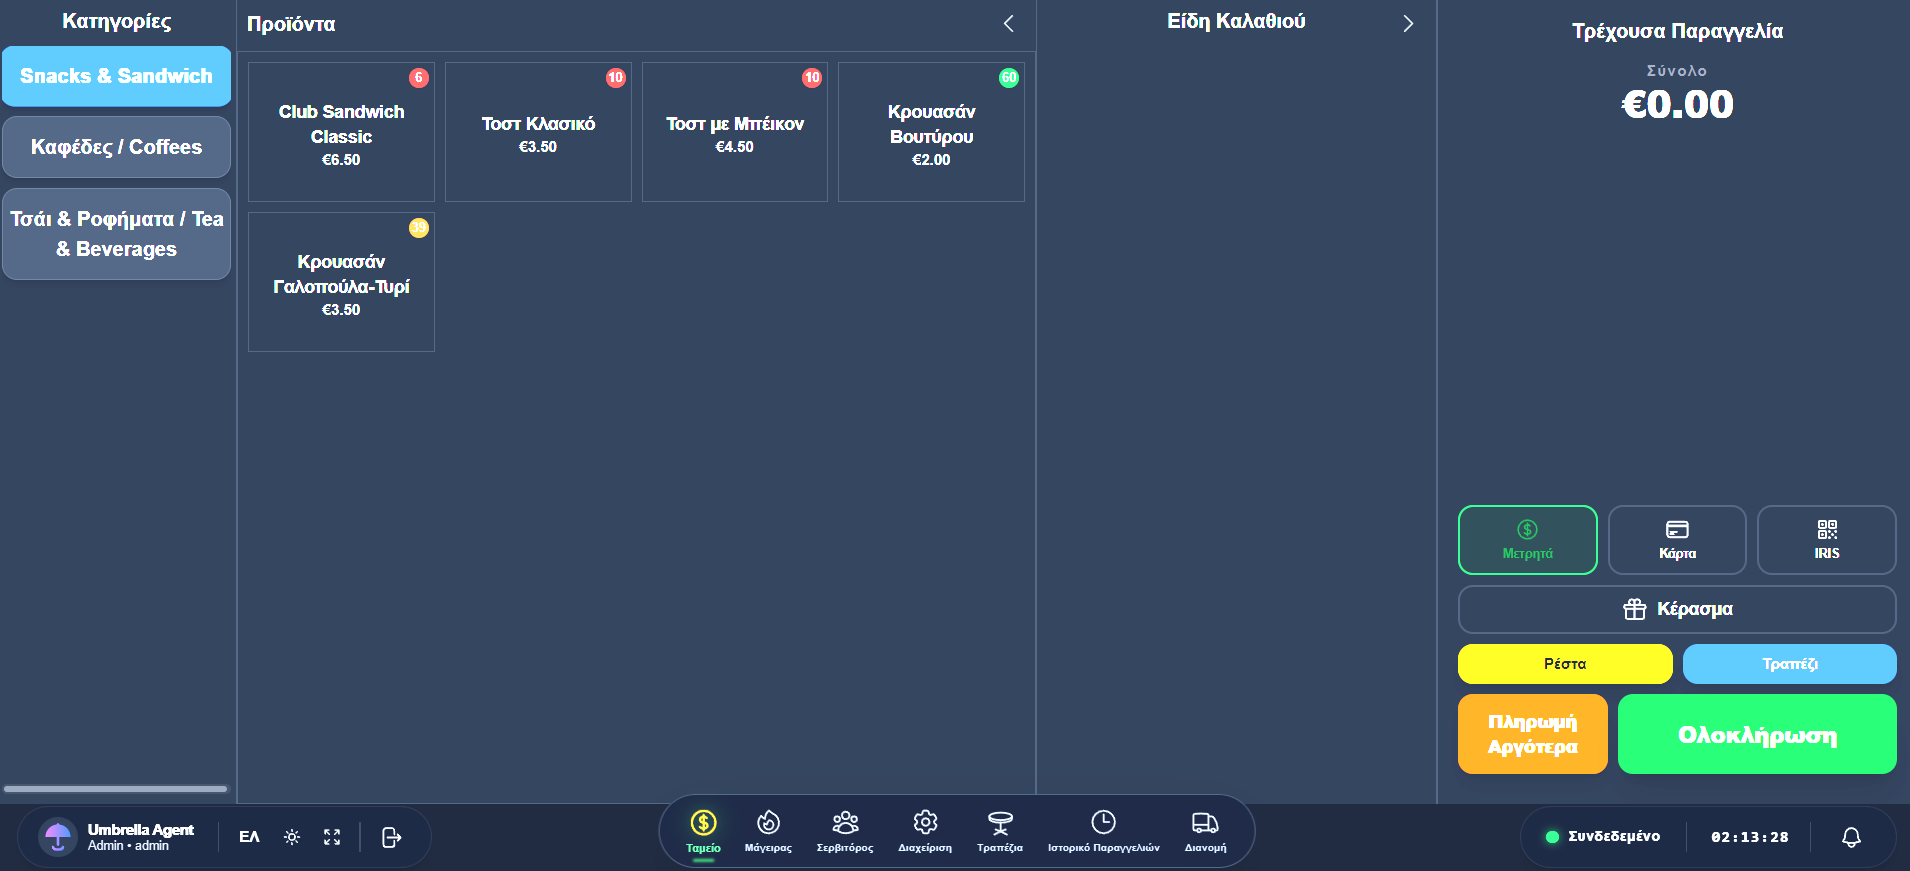
\includegraphics[width=1.0\textwidth]{images/ui_cashier.png}
    \caption{The primary Cashier interface, actively demonstrating the core transactional layout and Eclipse UI optical hierarchy.}
    \label{fig:ui_cashier}
\end{figure}

On the other hand, the kitchen interface (Figure~\ref{fig:ui_kitchen}) utilizes large high-contrast typography, negative space, and extremely peripheral vision-readable typography to eliminate all unnecessary aesthetics and maximize readability for the chef(s) who are likely to endure the greatest degree of pressure.

\begin{figure}[htbp]
    \centering
    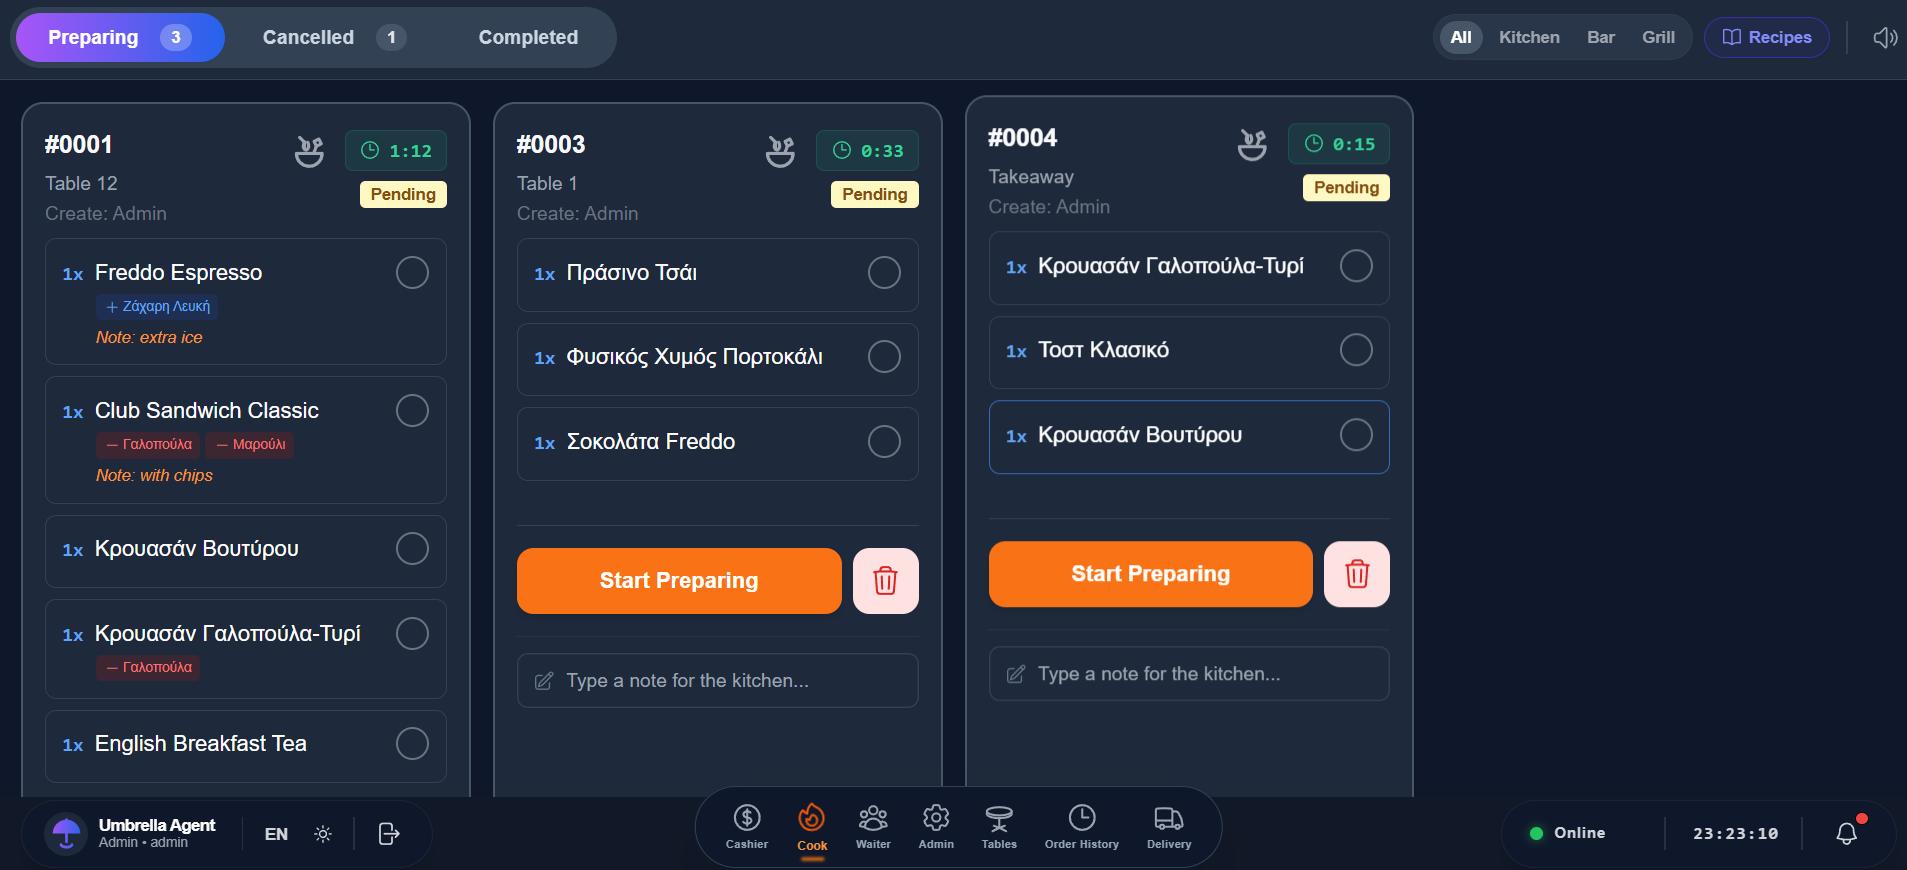
\includegraphics[width=1.0\textwidth]{images/ui_kitchen.png}
    \caption{The specialized kitchen interface, heavily optimized for high-contrast visibility and gross-motor interaction without requiring direct optical focus.}
    \label{fig:ui_kitchen}
\end{figure}

Lastly, the administrative dashboard is the central hub for the analytics toolsets and is capable of delivering simple, informative, and actionable chart visualization in near-real time by rapidly aggregating numerous transactions flowing through the underlying WebSocket infrastructure (See Figure~\ref{fig:ui_admin}).

\begin{figure}[htbp]
    \centering
    % TODO: Insert a screenshot of the Admin Stats Dashboard showing charts or metrics
    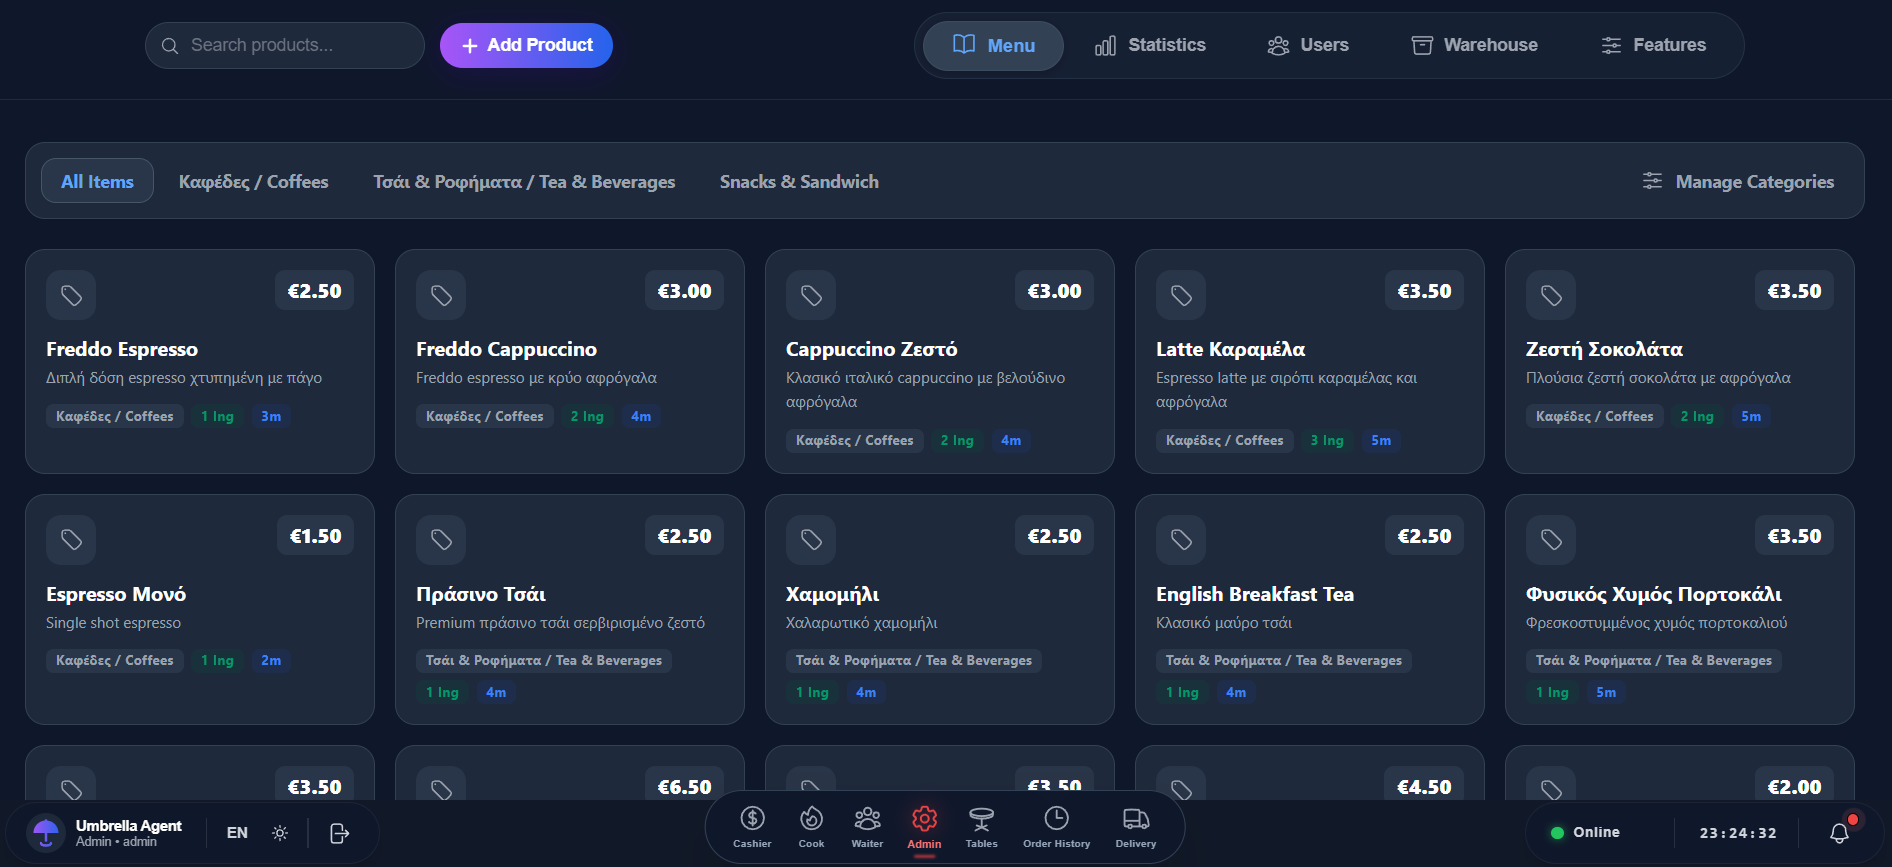
\includegraphics[width=1.0\textwidth]{images/ui_admin.png}
    \caption{The live Administrative Dashboard interface, projecting real-time aggregated financial and operational metrics.}
    \label{fig:ui_admin}
\end{figure}

\subsection{State Architecture Management Using the Virtual DOM}

Using the React framework, the positive effects of this method of rendering were greatly amplified by its built-in Virtual DOM \cite{freeman2019pro,nguyen2021,hunt2024reconciliation}. Upon receiving a WebSocket message informing the application that an order had been created, Zustand would update the entire application's global state in memory (the Zustand authentication store implementation is provided in Appendix~\ref{sec:code_zustand}). After updating the global state, React would compare it to the cached Virtual DOM tree. Rather than initiating the computationally intensive process of performing a browser-wide reflow to refresh the entire user interface, React would compute the minimum number of elements (or ``diff'') required for the new state to be rendered to the screen and then use those elements to perform surgical updates to only the relevant portions of the DOM (HTML). This provides users with a silky-smooth 60 FPS experience, even when there is extreme traffic or other operational spikes. Ultimately, these computed differences are used to create the new user interface state on the display. Therefore, the Virtual DOM ensures that no matter how much data is being pushed into the application via WebSocket broadcasts, the application will always provide a responsive and reliable 60 FPS experience.

\begin{figure}[htbp]
    \centering
    \centering
    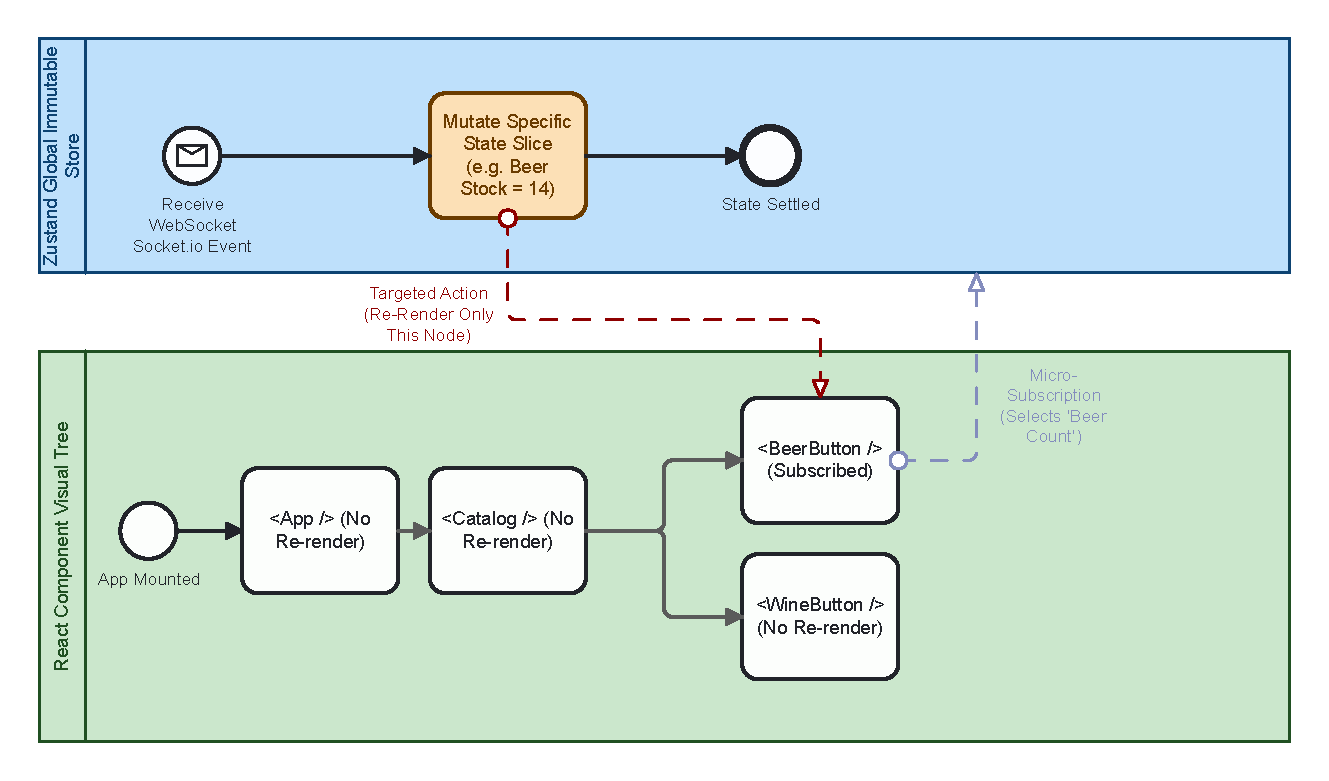
\includegraphics[width=0.8\textwidth]{images/ch4_zustand_flow.pdf}
    \caption{The unidirectional Zustand state management architecture, preventing expensive global re-renders upon real-time socket events.}
    \label{fig:zustand_architecture}
\end{figure}

\subsection{Overcoming Browser Limitations and The Autoplay Policy}

The major barrier to performing real-world field testing of the equipment was the ``autoplay'' restriction imposed on nearly all contemporary desktop and mobile web browsers (i.e., Google Chrome, Safari, etc.). Most desktop and mobile web browsers prohibit the programmatically initiated playback of audio content (for example, the critical audio signal to notify a busy cook of an incoming order) unless the audio content is first triggered by the users' own actions within the browser (e.g., tapping a physical button within the browser).
The ``autoplay'' restriction may also hinder the implementation of our system by simply placing the kitchen tablet on a high shelf in the kitchen awaiting a real-time notification to occur. When a real-time notification occurs simultaneously with the transmission of the notification from a cashier located on the opposite side of the festival grounds (possibly hundreds of meters away), the browser receives and then silently denies the programmatic audio call, based upon its determination that the audio call constitutes an unauthorized interruption. To circumvent this stringent protection mechanism without requiring a significant change to the present workflow for hands-off operation, we have created a silent unlock strategy that can operate in conjunction with the React lifecycle.
The silent unlock strategy is employed to unlock/authorize the browser's audio context for the entire duration of the session window of the browser that the chef uses to log onto the system upon the beginning of his/her working shift by instructing the system audio context to load and play a microsecond-long, zero-duration, completely silent audio file. This creative workaround to the browser's autoplay restriction allows the browser's audio context to remain enabled for the remainder of the current active session window, thereby allowing the audible and loud audio signals sent from the server via the WebSocket protocol to be audible during the full ten-hour length of the working shift, without requiring additional actions by the kitchen staff.

\section{Software Supply Chain and API Defense}

In this way, these are considered defensive layers to sanitize traffic going into your business logic layer. Strict auditing is enforced in our CI pipelines to aid in the prevention of software supply chain attacks \cite{sonatype2024supplychain}. To further limit the number of requests that an IP may send per second to our APIs, rate limiting has been added, thus providing a level of defense against basic Level 7 Distributed Denial of Service (DDoS) attacks. Input validation, along with parameterized database queries, have removed the risks associated with both standard NoSQL and SQL injection attacks \cite{owasp2025}. Due to the fact that we operate within a financial transaction environment, we treat all data as if it existed on a hostile public network. As such, we employ robust Zero Trust architecture principles \cite{nist2020zero}.

Helmet.js is utilized to implement a very restrictive Content Security Policy (CSP) header that eliminates XSS vectors through explicit denial of inline script executions \cite{google2016csp}. Helmet.js is also utilized to restrict autoplay policies to ensure that custom kitchen audio chimes will play instead of being blocked by modern browsers. Lastly, in order to provide additional defense mechanisms for potential complex SQL injection attacks at the application layer (e.g., sending an operator object instead of a string), sanitizing middleware has been applied to programmatically remove all special, reserved system characters from the incoming data stream, therefore preventing an executable command (disguising itself as user input) from ever reaching the database driver. The last defense mechanism implemented was adding another layer of protection to prevent user enumeration attacks during login processes. The authentication controller has been modified to return identical error messages and create identical processing delays due to security failures during both identification and password inputs.
